Let,
\begin{align} \label{eq:solutions/line_plane/70/codes/Assignment_2given}
    \frac{x-5}{3} = \frac{y+4}{7} = \frac{z-6}{2} = t
\end{align}

Equation of the line from the above \eqref{eq:solutions/line_plane/70/codes/Assignment_2given} can be expressed as,
\begin{align} \label{eq:solutions/line_plane/70/codes/Assignment_2parametricform}
\implies    \myvec{x \\ y \\ z} = \myvec{3t+5 \\ 7t-4 \\ 2t+6}
\end{align}

It can be further written as,
\begin{align} \label{eq:solutions/line_plane/70/codes/Assignment_2line_eq}
\implies    \textbf{x} = \myvec{5 \\ -4 \\ 6} + t\myvec{3 \\ 7 \\2}
\end{align}
where,
\begin{align} \label{eq:solutions/line_plane/70/codes/Assignment_2vector_x}
	\textbf{x} = \myvec{x \\ y \\ z}
\end{align}
Hence, equation \ref{eq:solutions/line_plane/70/codes/Assignment_2line_eq} gives the equation of a line and for t=0, the line passes through the point \myvec{5 \\ -4 \\ 6} \\
Plot of the line which passes through the point when t=0 is given below in Fig. \ref{myplot:solutions/line_plane/70/codes/Assignment_2}

\begin{figure}[h!]
\centering
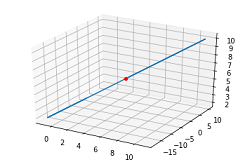
\includegraphics[width=\columnwidth]{./solutions/line_plane/70/codes/Assignment_2}  
\caption{Line passing through point (5,-4,6)}
\label{myplot:solutions/line_plane/70/codes/Assignment_2}
\end{figure}
